\section{Evaluation}
To investigate the effectiveness of our method, we evaluate our transfer learning based classification technique on actual data and point names of sensors from three commercial buildings. Extensive experiments demonstrate that our technique is able to accurately classify by type for a considerable portion of examples without human intervention. 
To further demonstrate what the technique is useful for, we combine the transfer learning with traditional labeling process to accelerate the learning speed.

\subsection{Taxonomy and Data Collection}
\begin{figure}[t]
\centering
\includegraphics[width=0.38\textwidth]{./fig/hvac}
\caption{A typical HVAC system consisting of an air handler unit (AHU), several variable air volume boxes (VAV), water-based heating/cooling pipes and air circulation ducts. (Figure used with permission from the authors of~\cite{sentinel}.)}
\label{fig:hvac}
\end{figure}

Figure~\ref{fig:hvac} illustrates a typical heating, ventilation, and air conditioning (HVAC) system deployed in modern commercial buildings. 
An HVAC system usually uses a combination of hot and cold water pipes in conjunction with
air handler units (AHU) to maintain the appropriate thermal environment within the building.
An HAVC system usually consists of several AHUs and each AHU is responsible for a physical zone
in the building. An AHU consists of variable speed drives that supply cold air
(cooled by the supplied cold water) using ducts to VAV boxes distributed throughout the building.
The hot water loop is also connected to these VAV boxes using separate pipes. Each VAV box
controls the amount of air to be let into an HVAC zone using dampers, whose opening angle
can be programmed. A reheat coil, which uses supplied hot water, is used to heat the air to
meet the appropriate HVAC settings for each zone.

Table~\ref{table:num} summarizes all the types of sensors evaluated in our analysis in these three buildings and the number of sensors of each type. ``Room temperature'' measures the temperature in room and for a better understanding, all the other temperature measurements on water circulation and air ventilation are illustrated in Figure~\ref{fig:hvac}. For setpoints, we assign only
one general type which includes all set points for every actuator configured in the building.

Our evaluation data set containing both data and point names of sensor streams is collected from over 2,500 sensors of different types deployed in three commercial buildings. 
We collected a week's worth of data from each building.
Specifically, Building A is the Rice Hall at the University of Virginia, where the sensing points report to a database by Trane anywhere between every 10 seconds to every 10 minutes.
Both building B and C are from UC Berkeley: B is the Sutardja Dai Hall with sensors and equipment from KETI\footnote{\url{http://www.keti.re.kr/}} and Siemens, while building C is the Soda Hall that uses an archaic system by Barrington Controls which is no longer in business. 
Points and sensors in these two buildings transmit data to an archiver~\cite{smap} periodically from anywhere between every 5 seconds to every 10 minutes.


\begin{table}[t]
\centering
\begin{tabular}{l | l l l}
\hline
& \multicolumn{3}{c}{Building} \\
Type & A & B & C\\
\hline\hline
$CO_{2}$ & 16 & 52 & 0\\
Humidity & 54 & 52 & 0\\
Air Pressure & 142 & 216 & 215\\
Room Temp & 159 & 231 & 208\\
Facility Operation Status & 59 & 72 & 41\\
Facility Control & 0 & 138 & 403\\
Setpoint & 140 & 486 & 229\\
Air Flow Volume & 14 & 172 & 9\\
Damper Position & 0 & 290 & 10\\
Fan Speed & 0 & 25 & 15\\
HW Supply Temp & 27 & 1 & 0\\
HW Return Temp & 15 & 1 & 0\\
CW Supply Temp & 18 & 2 & 11\\
CW Return Temp & 15 & 3 & 10\\
Supply Air Temp & 20 & 17 & 3\\
Return Air Temp & 6 & 2 & 4\\
Mixed Air Temp & 5 & 2 & 3\\
Ice Tank Entering Temp & 1 & 2 & 0\\
Ice Tank Leaving Temp & 1 & 4 & 0\\
Occupancy & 25 & 52 & 0\\
Timer & 0 & 0 & 15\\ \hline
Sum & 575 & 1124 & 1166\\ \hline
\end{tabular}
\caption{Number of points by type for the 3 test buildings. ``Temp" stands for ``temperature", ``HW" for ``hot water" and ``CW" for ``cold water".}
\label{table:num}
\end{table}


All of our learning and classification processes are implemented based on the scikit-learn~\cite{scikit} library, which is an open-source machine learning package 
implemented mostly in Python providing a rich set of APIs.

\subsection{Feature Transferability}
Now with the two different types of features explained, we examine how well both can perform in classifying sensor types when applied across buildings, i.e., learning a classifier based on the features from building A and testing it on building B. 
Intuitively, data features should be more generalizable than point names with respect to differentiating points by types. 
This is because in general a certain type of sensors will share commonality in reading amplitude and trend, such as diurnal patterns. 
For example, temperature readings in a building will be between 60-70 degree with rises in the morning and falls at night.
In contrast, point name features might not transfer well due to various naming conventions across buildings as shown in Table~\ref{table:ex}.
Although k-mers can enlarge the size of term dictionary in a building to increase the chance of covering more terms in other buildings, such a technique still cannot fundamentally compensate for the difference in naming conventions.

\begin{table}[h]
\centering
\begin{tabular}{l|c|c}
\hline
                & Data Feature & Name Feature \\ \hline
A-\textgreater B & 0.778       & 0.341       \\
B-\textgreater A & 0.612       & 0.328       \\ \hline
\end{tabular}
\caption{Type classification accuracy between two buildings with different sets of features.}
\label{table:clf}
\end{table}


To empirically examine how well each type of feature transfers, we perform type classification across buildings with both features in separate. With either set of features from building A, we train a linear SVM and apply it to building B on the same type of feature, or vice versa. Table~\ref{table:clf} summarizes the results.
We see that data features do transfer better than name features as expected, but the results from data features still contain significant errors making them far from being usable. 
The question remains how to better leverage these two sources of information from one building and transfer them to another.
We will discuss the idea of transfer learning in next section.

\subsection{Features for Clustering}
We use point name features to generate clusters for the new building. In general, point names following the same pattern would not vary too much, which will yield clusters of higher quality than data features.
Table~\ref{quality} shows the quality of clusters generated by DP with data features and name features measured by rand index~\cite{rand}. Rand index is a standard measure of the similarity between the grouping in clusters and the true labels.

\begin{table}[h]
\centering
\begin{tabular}{l|c|c}
\hline
                & Data Feature & Name Feature \\ \hline
Rand Index & 0.34       & 0.75       \\ \hline
\end{tabular}
\caption{Quality of clusters generated with different features measure by rand index (in the range [0,1], higher is better).}
\label{quality}
\end{table}

\subsection{Transfer Learning Performance}
\subsubsection{Base Classifiers and Performance}
\label{sec:baseline}
Our transfer learning based approach employs a few base classifiers. Each base classifier will be trained on the same set of data features from the source building in a general way, therefore there is no particular requirement on what classifiers should be selected here.
Particularly, we employ three base classifiers: random forest, linear regression and support vector machines with RBF kernels.


\begin{figure*}[ht!]
\centering
  \begin{subfigure}{0.32\textwidth}
                \centering
    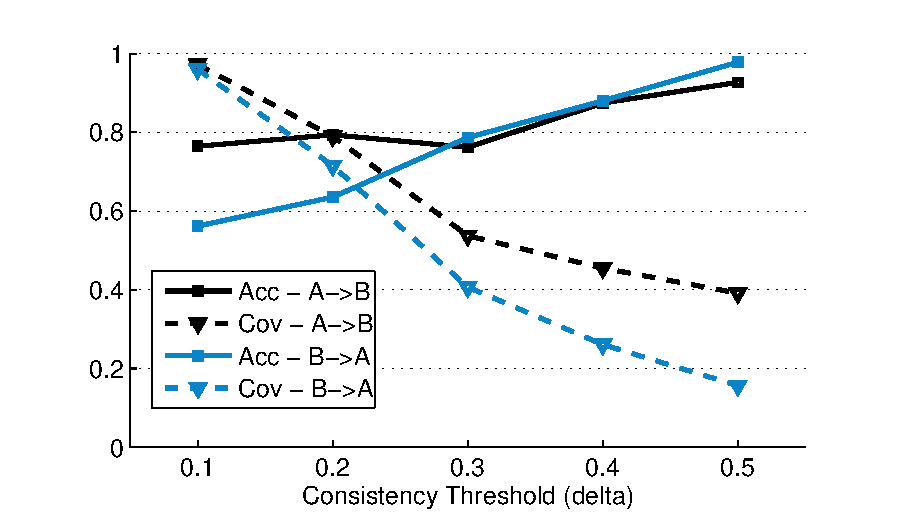
\includegraphics[width=\textwidth]{./fig/TL_AB.eps}
                \caption{A and B}
  \end{subfigure}
  \begin{subfigure}{0.32\textwidth}
                \centering
    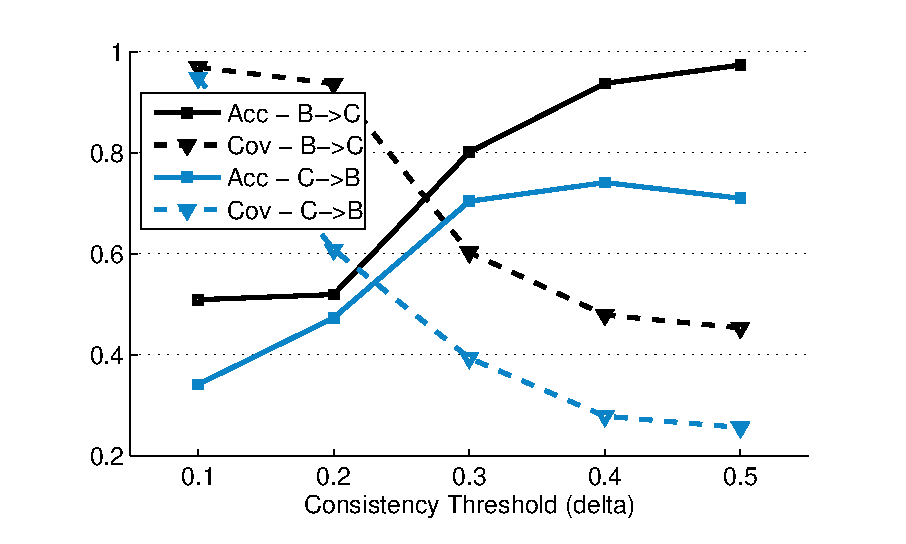
\includegraphics[width=\textwidth]{./fig/TL_BC.eps}
                \caption{B and C}
  \end{subfigure}
  \begin{subfigure}{0.32\textwidth}
                \centering
    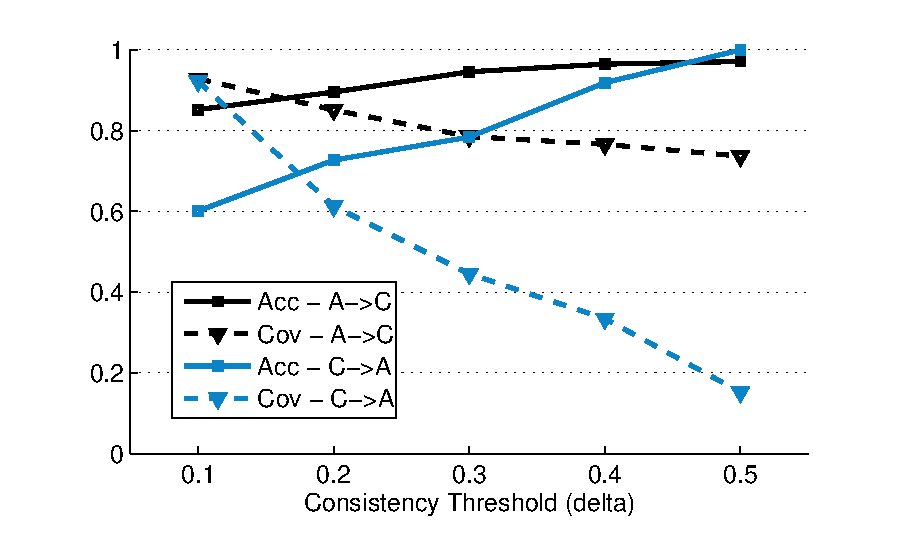
\includegraphics[width=\textwidth]{./fig/TL_AC.eps}
                \caption{A and C}
  \end{subfigure}
\caption{Type classification accuracy (Acc) against labeled percentage (Cov) with transfer learning between different pairs of buildings (denoted as X->Y). As we increase the threshold, the coverage drops while the overall accuracy increases. }
\label{fig:tl_acc}
\end{figure*}


\begin{table*}[]
\centering
\begin{tabular}{r|c|c|c}
\hline
 & Target A     & B     & C     \\ \hline
Source A & N/A   & 0.754/0.496/0.510 & 0.921/0.766/0.538 \\ \hline
B & 0.614/0.228/0.362 & N/A   & 0.513/0.247/0.258 \\ \hline
C & 0.582/0.299/0.421 & 0.393/0.158/0.190 & N/A   \\ \hline
\end{tabular}
\caption{Base classifier performance across buildings on data features. The three numbers are the accuracy for random forest, logistic regression and SVM respectively.}
\label{acc_base}
\end{table*}

\begin{table*}[]
\centering
\begin{tabular}{r|c|c|c|c|c|c}
\hline
\multirow{2}{*}{} & \multicolumn{2}{c|}{Target A} & \multicolumn{2}{c|}{B} & \multicolumn{2}{c}{C} \\ \cline{2-7} 
                  & Acc        & F1        & Acc        & F1        & Acc        & F1        \\ \hline
Source A                 & N/A      & N/A     & 0.943/0.934      & 0.936/0.931     & 0.977/0.970      & 0.981/0.971     \\ \hline
B                 & 0.897/0.875     & 0.932/0.913     & N/A      & N/A     & 0.950/0.952      & 0.939/0.937     \\ \hline
C                 & 0.862/0.862     & 0.864/0.864     & 0.726/0.702      & 0.691/0.726     & N/A     & N/A     \\ \hline
\end{tabular}
\caption{Accuracy and F1 score of transfer learning and the best baseline with $\delta$=0.4. Each cell contains two numbers for our approach and the baseline respectively. Overall, our approach outperforms the baseline.}
\label{table:f1}
\end{table*}

For the three buildings, we have three pairs of choices and for each pair the training/testing can be conducted either way - therefore, we have six testing cases.
The performance of the base classifiers when applied across buildings is shown in Table~\ref{acc_base}, the base classifiers achieve the accuracy anywhere between 0.158 and 0.921.
INSIGHT.

\subsubsection{Single Building as the Source}
We first consider the case where only one building is exploited as the knowledge transfer source, i.e., each base classifier is trained on data from only one building. 
The overall accuracy of transfer learning for type classification across our three testing buildings are illustrated in Figure~\ref{fig:tl_acc}.
There is an intrinsic trade-off between the prediction accuracy and the percentage being labeled, since we set a threshold on the average weight of base classifiers. 
As expected, when we increase the threshold $\delta$ on the average weight for base classifiers, we have labels of better quality with a drop in the percentage of examples being labeled. Empirically, we can set a threshold $\delta$ around 0.4, which strikes a reasonable balance between accuracy and coverage.

On such imbalanced data sets, investigation of accuracy only is not enough. We also measure the weighted macro F1 score of classification for our approach and the baseline. The weighted macro F1 score is an altered version of macro F1 score~\cite{yang}, which calculates the F1 score for each class, where ``one-versus-all'' binary classification is performed, and weight the resulting F1 of each class by support (the number of true instances for each label). 

As a baseline to compare our proposed approach against, we take the subset of examples in the new building that get labeled by the transfer learning process, and apply the base classifiers to predict labels on the same subset. 
Particularly, we take the choice of 0.4 for the threshold $\delta$ and apply the base classiifers to predict labels for the same subset that gets labeled by the transfer learning process. We repeat 10 times for the experiment in each direction (e.g., A->B) and the average of the resuls is reported in Table~\ref{table:f1}. 
INSIGHT.
%Paired two sample t-test is performed to validate the statistical significance of improvement from our method over the best-performing baseline. 
\subsubsection{Multiple Buildings as the Source}
\begin{table}[h]
\centering
\begin{tabular}{r|cc|cc}
\hline
\multirow{2}{*}{} & \multicolumn{2}{c|}{Two Sources} & \multicolumn{2}{c}{Single Source} \\ \cline{2-5} 
 & Acc & Cov & Acc & Cov \\ \hline
Target A & 0.863 & 0.397 & 0.855 & 0.362 \\ \hline
B & 0.899 & 0.458 & 0.874 & 0.455 \\ \hline
C & 0.963 & 0.897 & 0.965 & 0.766 \\ \hline
\end{tabular}
\caption{Combining the knowledge from multiple buildings to infer on the new one is superior to exploiting one source building.}
\label{2source}
\end{table}

In practice, it is common to have labels for multiple buildings available and combining them all as the source to transfer knowledge is expected to achieve better performance.
To verify the effectiveness of using multiple buildings as the source, we repeat the above experiments with two buildings as the training source for the other building. From Table~\ref{2source}, we see that combining multiple buildings as the source is superior to single source, as expected.

\subsection{Complementing Traditional Labeling}
Our method is designed to complement the traditional labeling techniques, rather then replacing them.
With a considerable percentage automatically labeled by our technique as a first step, the labeling process of a new building is expected to be accelerated significantly.
As a showcase, we adopt the technique developed in~\cite{cikm} and examine how much our technique can accelerate the labeling process.
%~\cite{cikm} formulates a clustering-based active learning approach to iteratively label the type of sensors, where they acquire human label for a ``representative'' example in each iteration and propagate the label to adjacent examples.
For brevity, we refer interested readers to~\cite{cikm} for the detail of their algorithm.

\begin{figure}[t]
\centering
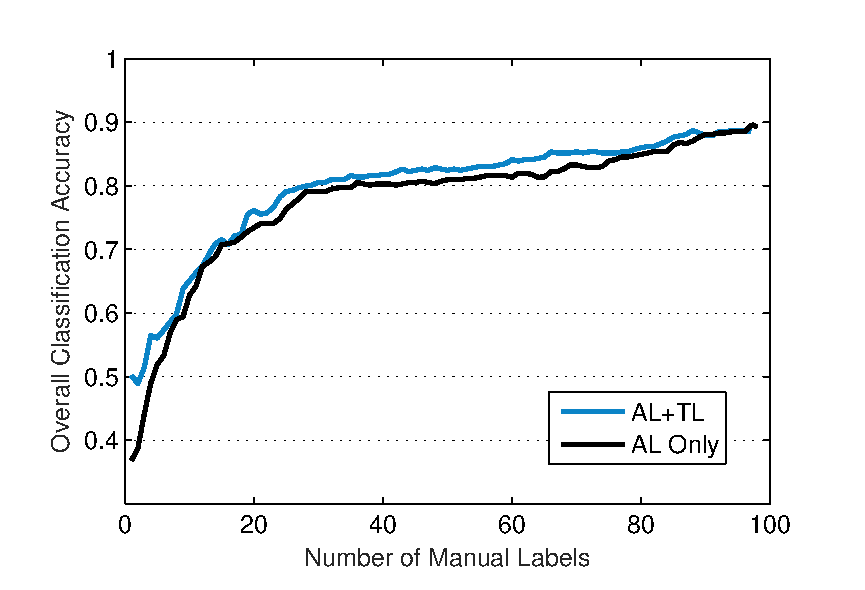
\includegraphics[width=0.4\textwidth]{./fig/tl_al.eps}
\caption{Our transfer learning based approach can complement traditional labeling technique to achieve faster coverage.}
\label{fig:comp}
\end{figure}


\subsection{Discussion}
%\paragraph{Unlabeled Streams}
%With a threshold on the average weight of base classifiers, our transfer learning based technique is able to label a portion of the streams in the new building, which leaves many unlabeled.
%The coverage might be increased by searching for the nearest neighbors in a certain radius to those unlabeled and combine them.
\paragraph{Number of Clusters}
Although we appeal to a non-parametric Bayesion clustering method in our algorithm to generate clusters on the testing building, we further justify such a choice by demonstrating how sensitive the transfer learning can be to the number of clusters generated.

\paragraph{Better Features for Classifiers} The performance of transfer learning and classification processes in our work is bounded by the base classifiers which rely only on a set of general features. The line of work to represent time series with discretized symbols (e.g., the SAX~\cite{sax}) or primitive ``shapes'' (e.g., the ``shapelets''~\cite{shapelet1, shapelet2}) doesn't work well for our problem due to the variability in ``shapes'' and unpredictable ``noises''. We wish to explore how using external or domain-specific knowledge could help improve the classification accuracy. 

